\documentclass[border=10pt]{standalone}
\usepackage{pgfplots}
\pgfplotsset{compat=1.18}
\begin{document}
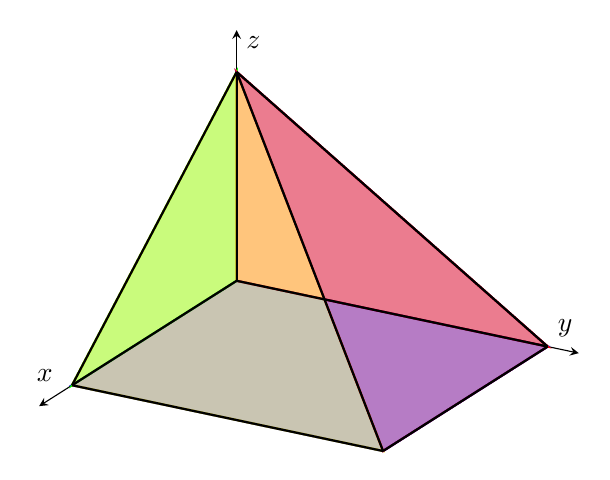
\begin{tikzpicture}
\begin{axis}[
    view={120}{30},
    xlabel={$x$},
    ylabel={$y$},
    zlabel={$z$},
    xmin=0, xmax=1.2,
    ymin=0, ymax=2.2,
    zmin=0, zmax=1.2,
    axis lines=center,
    grid=major,
    ticks=none
]
% Vertices
% V0: (0,0,0)
% V1: (1,0,0)
% V2: (1,2,0)
% V3: (0,2,0)
% V4: (0,0,1)

% Faces
% Face 1: z=0 (Base)
\addplot3[fill=blue, fill opacity=0.3, draw=blue, thick] coordinates {(0,0,0) (1,0,0) (1,2,0) (0,2,0) (0,0,0)};

% Face 2: y=0 (Side)
\addplot3[fill=green, fill opacity=0.3, draw=green, thick] coordinates {(0,0,0) (1,0,0) (0,0,1) (0,0,0)};

% Face 3: x=0 (Side)
\addplot3[fill=red, fill opacity=0.3, draw=red, thick] coordinates {(0,0,0) (0,2,0) (0,0,1) (0,0,0)};

% Face 4: x+z=1 (Side)
\addplot3[fill=yellow, fill opacity=0.3, draw=yellow, thick] coordinates {(1,0,0) (1,2,0) (0,0,1) (1,0,0)};

% Face 5: y+2z=2 (Side)
\addplot3[fill=purple, fill opacity=0.3, draw=purple, thick] coordinates {(0,2,0) (1,2,0) (0,0,1) (0,2,0)};

% Edges for extra definition
\draw[black, thick] (axis cs:0,0,0) -- (axis cs:1,0,0);
\draw[black, thick] (axis cs:1,0,0) -- (axis cs:1,2,0);
\draw[black, thick] (axis cs:1,2,0) -- (axis cs:0,2,0);
\draw[black, thick] (axis cs:0,2,0) -- (axis cs:0,0,0);
\draw[black, thick] (axis cs:0,0,0) -- (axis cs:0,0,1);
\draw[black, thick] (axis cs:1,0,0) -- (axis cs:0,0,1);
\draw[black, thick] (axis cs:1,2,0) -- (axis cs:0,0,1);
\draw[black, thick] (axis cs:0,2,0) -- (axis cs:0,0,1);

\end{axis}
\end{tikzpicture}
\end{document}
